\section{Introduction}

%%Introducing codon models and their usefulness
Phylogenetic codon models are now routinely used in many domains of bioinformatics and molecular evolutionary studies.
Most often used to characterize the genes, sites~\citep{Nielsen1998}, or lineages~\citep{Zhang2004} having experienced positive selection.
More generally, these models highlight the respective contributions of mutation, selection, genetic drift and biased gene conversion~\citep{Kosiol2019}, and the causes of their variation between genes~\citep{Zhang2015} or across species~\citep{Lartillot2011}.

%introducing the idea of a single $\omega$
Conceptually, codon models take advantage of the fact that synonymous and non-synonymous substitutions are differentially impacted by selection.
Assuming synonymous mutations are neutral, the synonymous substitution rate equal to the underlying mutation rate~\citep{kimura1983neutral}.
Non-synonymous substitutions, on the other hand, reflect the combined effect of mutation and selection~\citep{Ohta1995}.
Classical codon models formalize this idea by invoking a single parameter $\omega$, acting multiplicatively on non-synonymous substitutions rates~\citep{Muse1994, Goldman1994}.
Using a parametric model automatically corrects for the multiplicity issues created by the complex structure of the genetic code and by uneven mutation rates between nucleotides.
As a result, this parameter $\omega$ capture the net, or aggregate, effect of selection on non-synonymous mutations.

%elaborating on the phenomenological versus mechanistic, classical versus mutsel, distinction
Classical codon models, so defined, are phenomenological, they capture a complex mixture of selective effects through a single parameter~\citep{Rodrigue2010a}.
In reality, the selective effects associated with non-synonymous mutations depend on the context (site-specificity) and the amino acids involved in the transition~\citep{Kosiol2007}.
Attempts at an explicitly modelling of these complex selective landscapes have been formulated, named mechanistic codon models, based on the mutation-selection formalism~\citep{Halpern1998}.
However, these models are computationally complex~\citep{Rodrigue2010, Tamuri2012}, and classical codon models therefore remain an attractive, potentially more robust, although still perfectible, approach.

%bringing in the key issue here: correctly teasing apart mutation and selection
The parametric design of current classical models relying on aggregates parameters raises an important question.
By capturing selection through a single parameter, $\omega$, is the mutational process estimated reliably?
There are indications that this is not the case.
In their simplest form~\citep{Muse1994}, classical codon models predict that the nucleotide composition should be the same for all three positions of the codons, and should be equal to the nucleotide equilibrium frequencies implied by the underlying nucleotide substitution rate matrix.
In reality, composition differ, the third position shows more extreme composition, reflecting the underlying mutation bias, compared to first and second positions, which are typically closer to 50\% GC~\citep{Singer2000}.

%Ici, je pense qu’il faut un peu développer sur le formalisme 3x4, qui est directement pertinent
These modulations across the three coding positions have been accommodated using the so-called 3x4 formalism~\citep{Goldman1994, Pond2005a}, allowing for different nucleotide rate matrices at the three positions.
However, this is also problematic, since this modelling approach has the consequence that synonymous substitutions, say, from A to C, occur at different rates at the first and third positions.
Yet, in reality, the mutation process is blind to the coding structure, and should be homogeneous across coding positions, and if neutral, all mutations from A to C should have the same rate.

%Potential impact of these problems: both practical and conceptual
In any case, these observations suggest that the mutation matrix (1x4) or matrices (3x4) estimated by codon models are not correctly reflecting the mutation rates between nucleotides~\citep{Rodrigue2008a}.
Instead, what these matrices are capturing is the result of the compromise between mutation and selection at the level of the realized nucleotide frequencies.
For detecting selection, this problem is probably minor, although still bears consequences on the estimation of $\omega$~\citep{Spielman2015}.
Conceptually, however, this is a clear symptom of a more fundamental problem: mutation rates and fixation probabilities are not correctly teased apart.

Practically, this misconception could have important consequences in other contexts than tests of positive selection.
In particular, there is a current interest in investigating the variation between species in GC content, and its effect on the evolution of protein-coding sequences~\citep{Bolivar2019}.
An important factor here is biased gene conversion toward GC (named gBGC), which can confound the tests for detecting positive selection~\citep{Galtier2009,Ratnakumar2010, Figuet2014}.
Even in the absence of \acrshort{gBGC}, however, uneven mutation rates, varying across species, can have an important impact on the estimation of the strength of selection.
All this suggests that, even before introducing \acrshort{gBGC} in codon models, correctly formalizing the interplay between mutation and selection in current codon models would be an important thing to do.

%The mut-sel balance revisited: an equilibrium between two net forces
In this direction, the key point that needs to be correctly formalized is that the nucleotide's realized frequencies are the result of a compromise between mutation and selection, then this implies that the strength of selection is not the same between all nucleotide or amino-acid pairs.
For instance, if the mutation process is AT-biased, because of selection, the realized nucleotide frequencies at equilibrium will be less AT-biased than expected under the mutation process.
However, this implies that, at equilibrium, there will be a net mutation pressure toward AT, which has to be compensated for by a net selection differential toward GC, or, in other words, that mutations toward AT will be more deleterious on average than those toward GC.

%introducing $\omega$ as a tensor
All this suggests that, in order for a codon model to correctly formalize this subtle interplay between mutation and selection, the component of the parameter vector responsible for absorbing the net effect of selection (i.e. $\omega$) should not be a scalar, as is currently the case.
Instead, it should be a tensor, an array of $\omega$ values unfolding along multiple directions.
What is the parametric structure being able correctly tease apart mutation rates and selection, and this, without having to explicitly model the underlying fitness landscape?

%end of introduction: outline of the mean-field approach and of the results — à compléter à la fin
In the present work, we address this question.
In order to derive a codon model along those lines, our strategy is to first assume a true site-specific evolutionary process, following the mutation-selection formalism.
Then, we derive the mean substitution process implied across all sites by this mechanistic model.
Inferring parameters on simulated alignments, we show that the model correctly estimates the mutation rates.

% Improved inference of site-specific positive selection under a generalized parametric codon model when there are multinucleotide mutations and multiple nonsynonymous rates~\citep{Dunn2019}.
% Influence of mutation bias and hydrophobicity on the substitution rates and sequence entropies of protein evolution~\citep{Santos2018}.


\section{Results}
\label{sec:results}

We first conduct simulation experiments with a mutation-selection substitution model of site-specific amino-acid fitness landscape, based on two parameters tuning the mutation bias and the stringency of selection.
In section~\ref{subsec:simulations-experiments}, we explore through summary statistics the intricate interplay between mutation and selection in simulated experiments.
Then, in section~\ref{subsec:parameter-inference-on-simulated-data}, we explore how codon models with different parameterizations are able to infer the mutation and selection of the evolutionary process, tested on simulated alignments.
This model is subsequently applied to empirical alignments in section~\ref{subsec:estimation-of-empirical-sequence-data}.

\subsection{Simulations experiments}
\label{subsec:simulations-experiments}

Simulations of protein-coding \acrshort{DNA} sequences were conducted under an origin-fixation substitution process~\citep{McCandlish2014} at the level of codons.
In this context, mutations are defined at the level of nucleotides with a single parameter controlling mutational bias toward AT, denoted $\lambda = (\mutequi_A+\mutequi_T)/(\mutequi_C+\mutequi_G)$, which is shared by all sites of the sequence (see section~\ref{sec:mut-bias-mut-matrix}).
With regards to selection, synonymous mutations are considered neutral, such that the synonymous substitution rate equal to the underlying mutation rate.
Alternatively, selection is modelled for non-synonymous mutations, with site-specific amino-acid fitness profiles (i.e. a vector of 20 fitnesses for each codon site), drawn from a Dirichlet distribution of concentration parameter $\alpha$ (see section~\ref{sec:mut-bias-aa-selection}).
A low parameter $\alpha$ implies that each site-specific profile randomly drawn is likely uneven, with some amino acids with high fitness while other are with low fitness (for each site of the sequence).
Ultimately, the stringency of selection increase with decreasing $\alpha$.
Altogether, two parameters are necessary to tune the mutation bias ($\lambda$) and the stringency of selection ($\alpha$), as depicted in figure~\ref{fig:mut-bias-parameters}.

\begin{figure}[htbp]
    \centering
    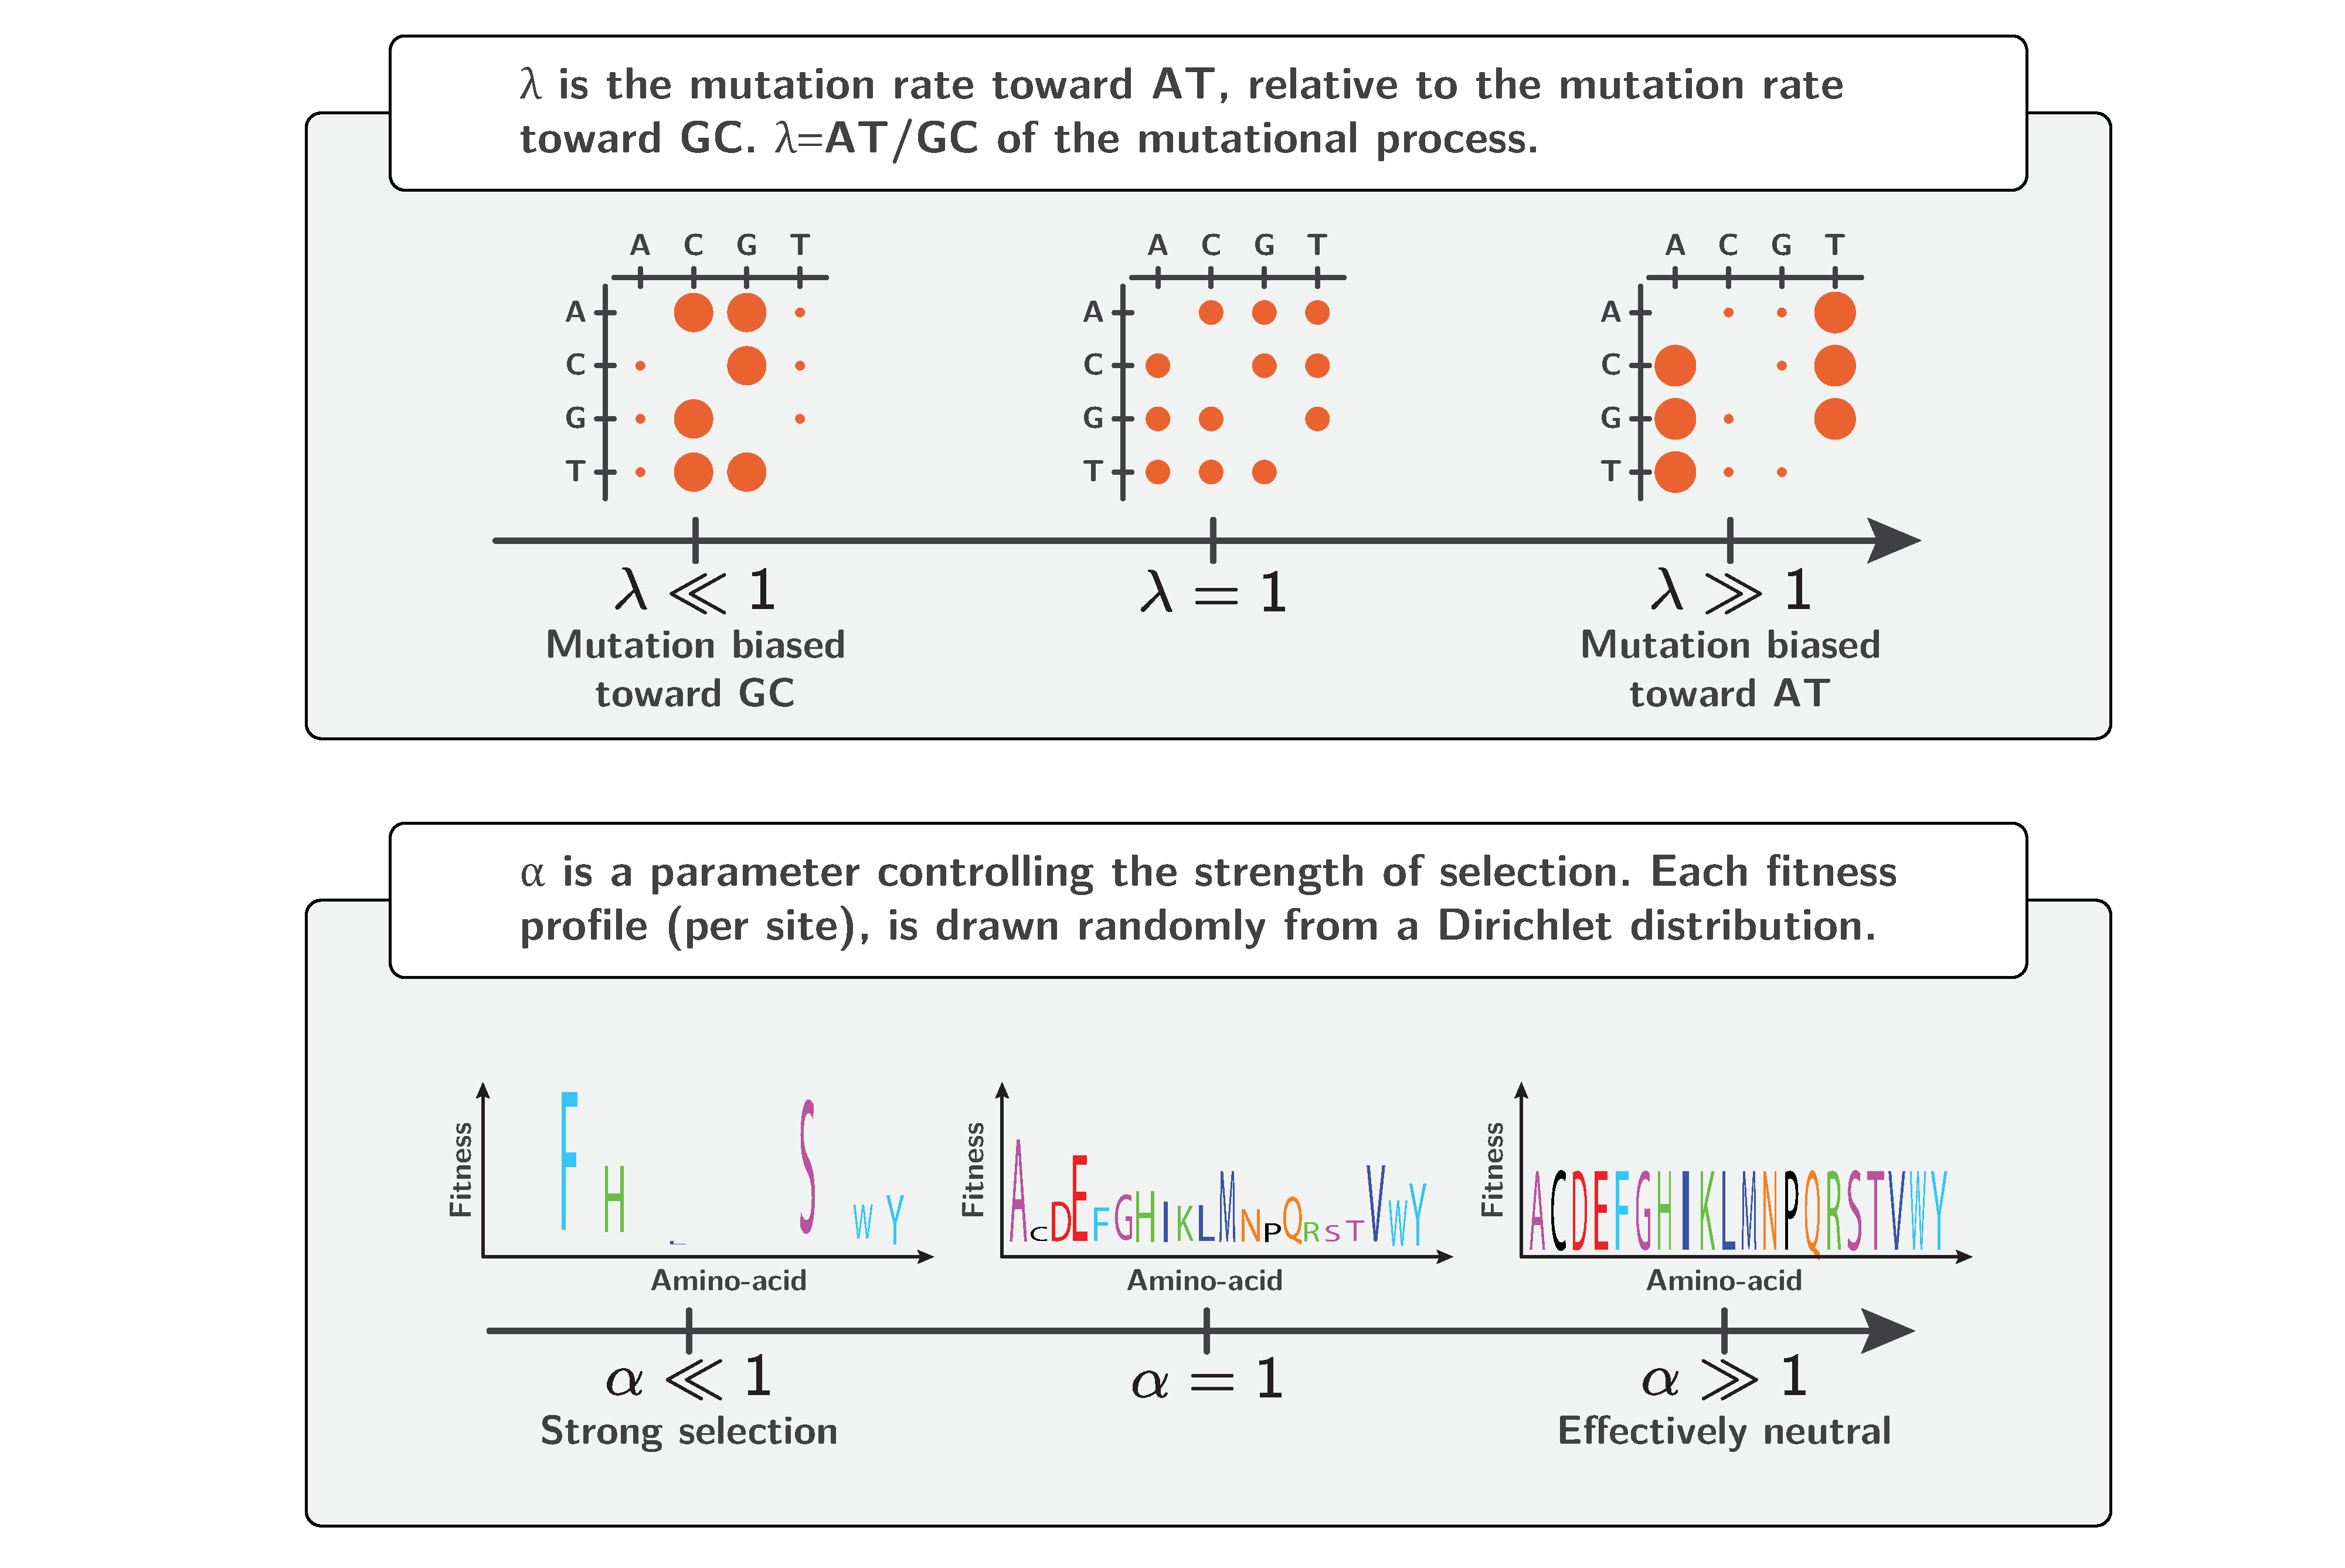
\includegraphics[width=\textwidth] {parameters}
    \caption[Parameters of the mutation-selection model]{
    Parameters of the mutation-selection model.
    Mutational bias (toward A and T) is shared by all sites of the sequence, and tuned by the parameter $\lambda$.
    Conversely, each codon site of the sequence is defined by a unique fitness profile, drawn from a Dirichlet distribution with concentration parameter $\alpha$.
    Stringency of selection increase with decreasing $\alpha$.}
    \label{fig:mut-bias-parameters}
\end{figure}

Simulation of this origin-fixation process along a species tree result in a multiple sequence alignment of \acrshort{DNA} for the extant species (see section~\ref{sec:mut-bias-simu}), from which summary statistics can be computed.
One such straightforward summary statistic is the frequency of the different nucleotides, and the resulting observed mutational bias $\atgc$ of the alignment.
Such observed mutational bias is compared to underlying mutational bias $\lambda$ at different positions of the codon (first, second and third), shown in figure~\ref{fig:mut-bias-AT-GC-obs}.
The third position of codons reflects the underlying mutational bias, while the first and second positions are impacted by the strength of selection and display less extreme bias than the underlying mutational bias.
This effect is explained by nucleotide mutations at the third codon position being more often synonymous, while mutations at first and second positions are more often changing the amino-acid and are more prone to selection.

\begin{figure}[htbp]
    \centering
    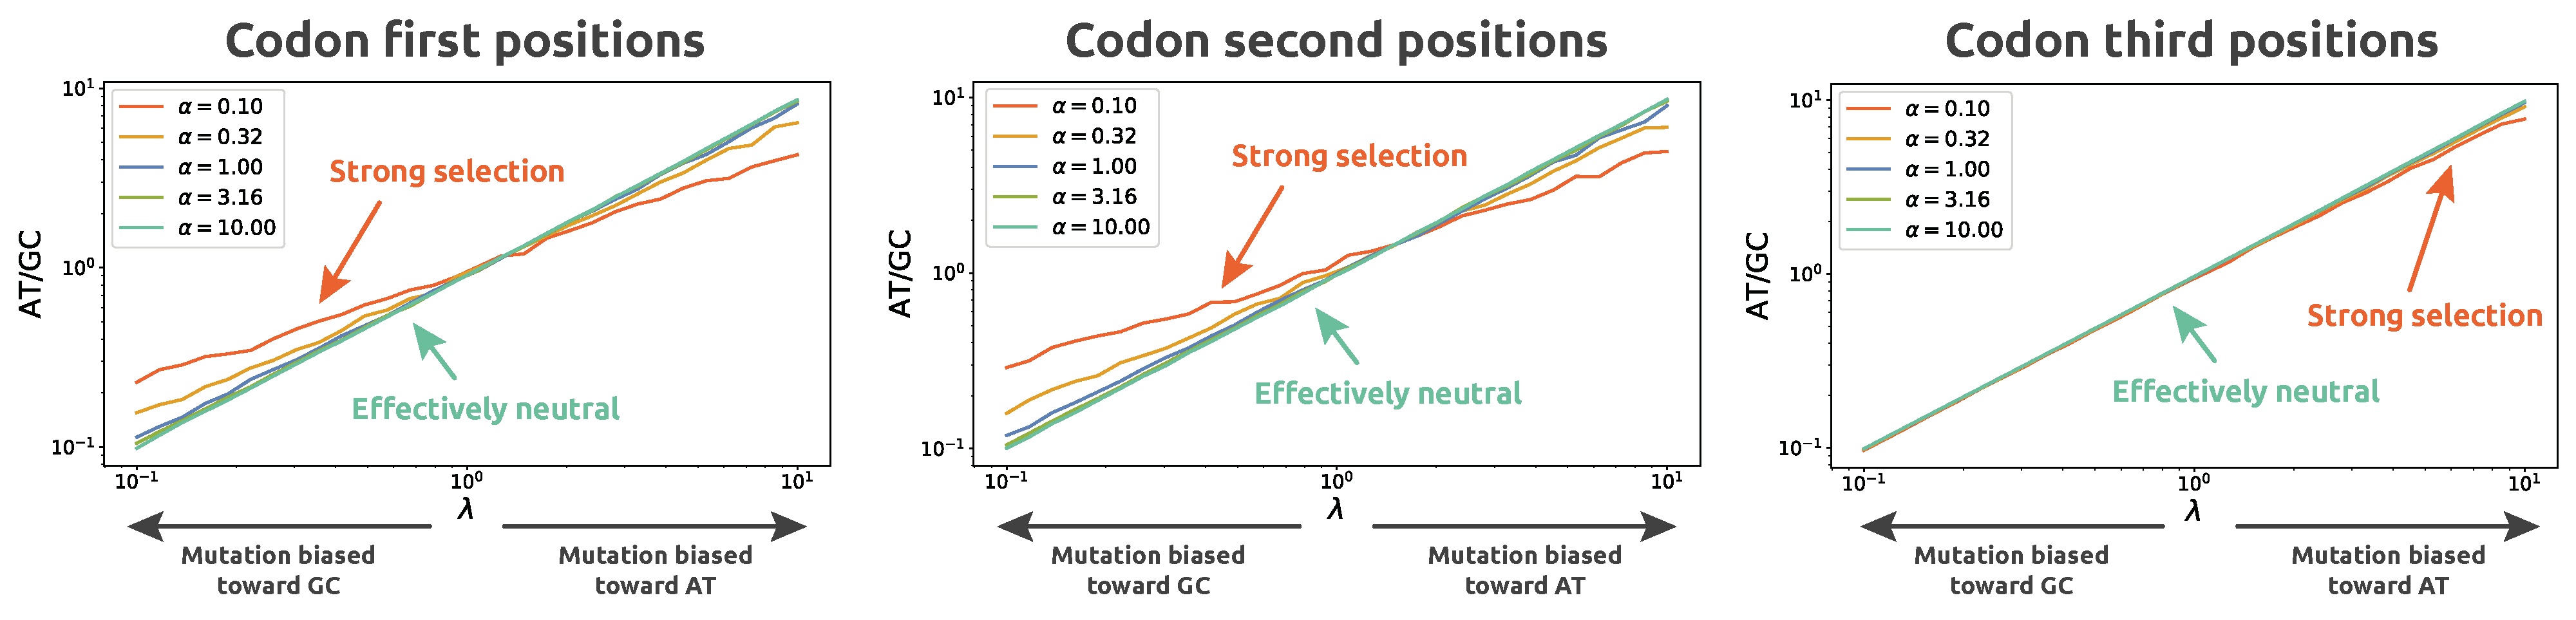
\includegraphics[width=\textwidth] {AT-GC-obs}
    \caption[$\atgc$ composition of the alignment]{
    Observed $\atgc$ composition of the alignment, represented at the different positions of codons (first, second and third), summed over all sites.
    The horizontal axis represents the underlying mutational bias ($\lambda$) of the nucleotide matrix, and the vertical axis represent the observed $\atgc$ of the codon position across the alignment.
    Stringency of selection is represented by 5 coloured solid lines with decreasing $\alpha$.
    $\atgc$ at the third codon position matches the mutational bias, whereas in contrast first and second positions are less extreme than the underlying bias.
    With increase stringency of selection (i.e. with decreasing $\alpha$), the observed bias is less reflecting the underlying mutational bias, such that selection is opposing the mutational bias.}
    \label{fig:mut-bias-AT-GC-obs}
\end{figure}

Beside the observed mutational bias of the alignment, the diversity of amino acids is an important indicator of the selective constraints that the sequence experiences.
This diversity is quantified by the frequencies of amino acids observed across all taxa in the alignment, summarized through a single statistic, namely the Shannon's entropy of amino-acid frequencies~\citep{Goldstein2017}, as described in section~\ref{subsec:entropy}.
Diversity can be quantified for a given site of the sequence, and this site-specific diversity can subsequently be averaged over all sites of the sequence.
Alternatively, the diversity can be quantified directly on the whole sequence by the observed amino-acid frequencies in the alignment.
These two variants of diversity are computed for alignment under different values of $\alpha$ and $\lambda$, presented in figure~\ref{fig:mut-bias-diversity-aa}.
Under stringent selection, only a small number of amino acids are actually permissible any given site resulting in low site-specific diversity.
Yet all amino acids occur at comparable frequencies in the alignment resulting in high sequence diversity.
These observations highlight the distinction between averaged site-specific diversity and sequence diversity.
Moreover, the mutational bias (either toward AT or toward GC) greatly reduces both site-specific and sequence diversity, such that the composition of amino acids is highly dependent on the underlying mutational bias.
This effect is less visible whenever selection is more stringent (i.e. with decreasing $\alpha$), but can still be observed even for stringent selection.

\begin{figure}[htbp]
    \centering
    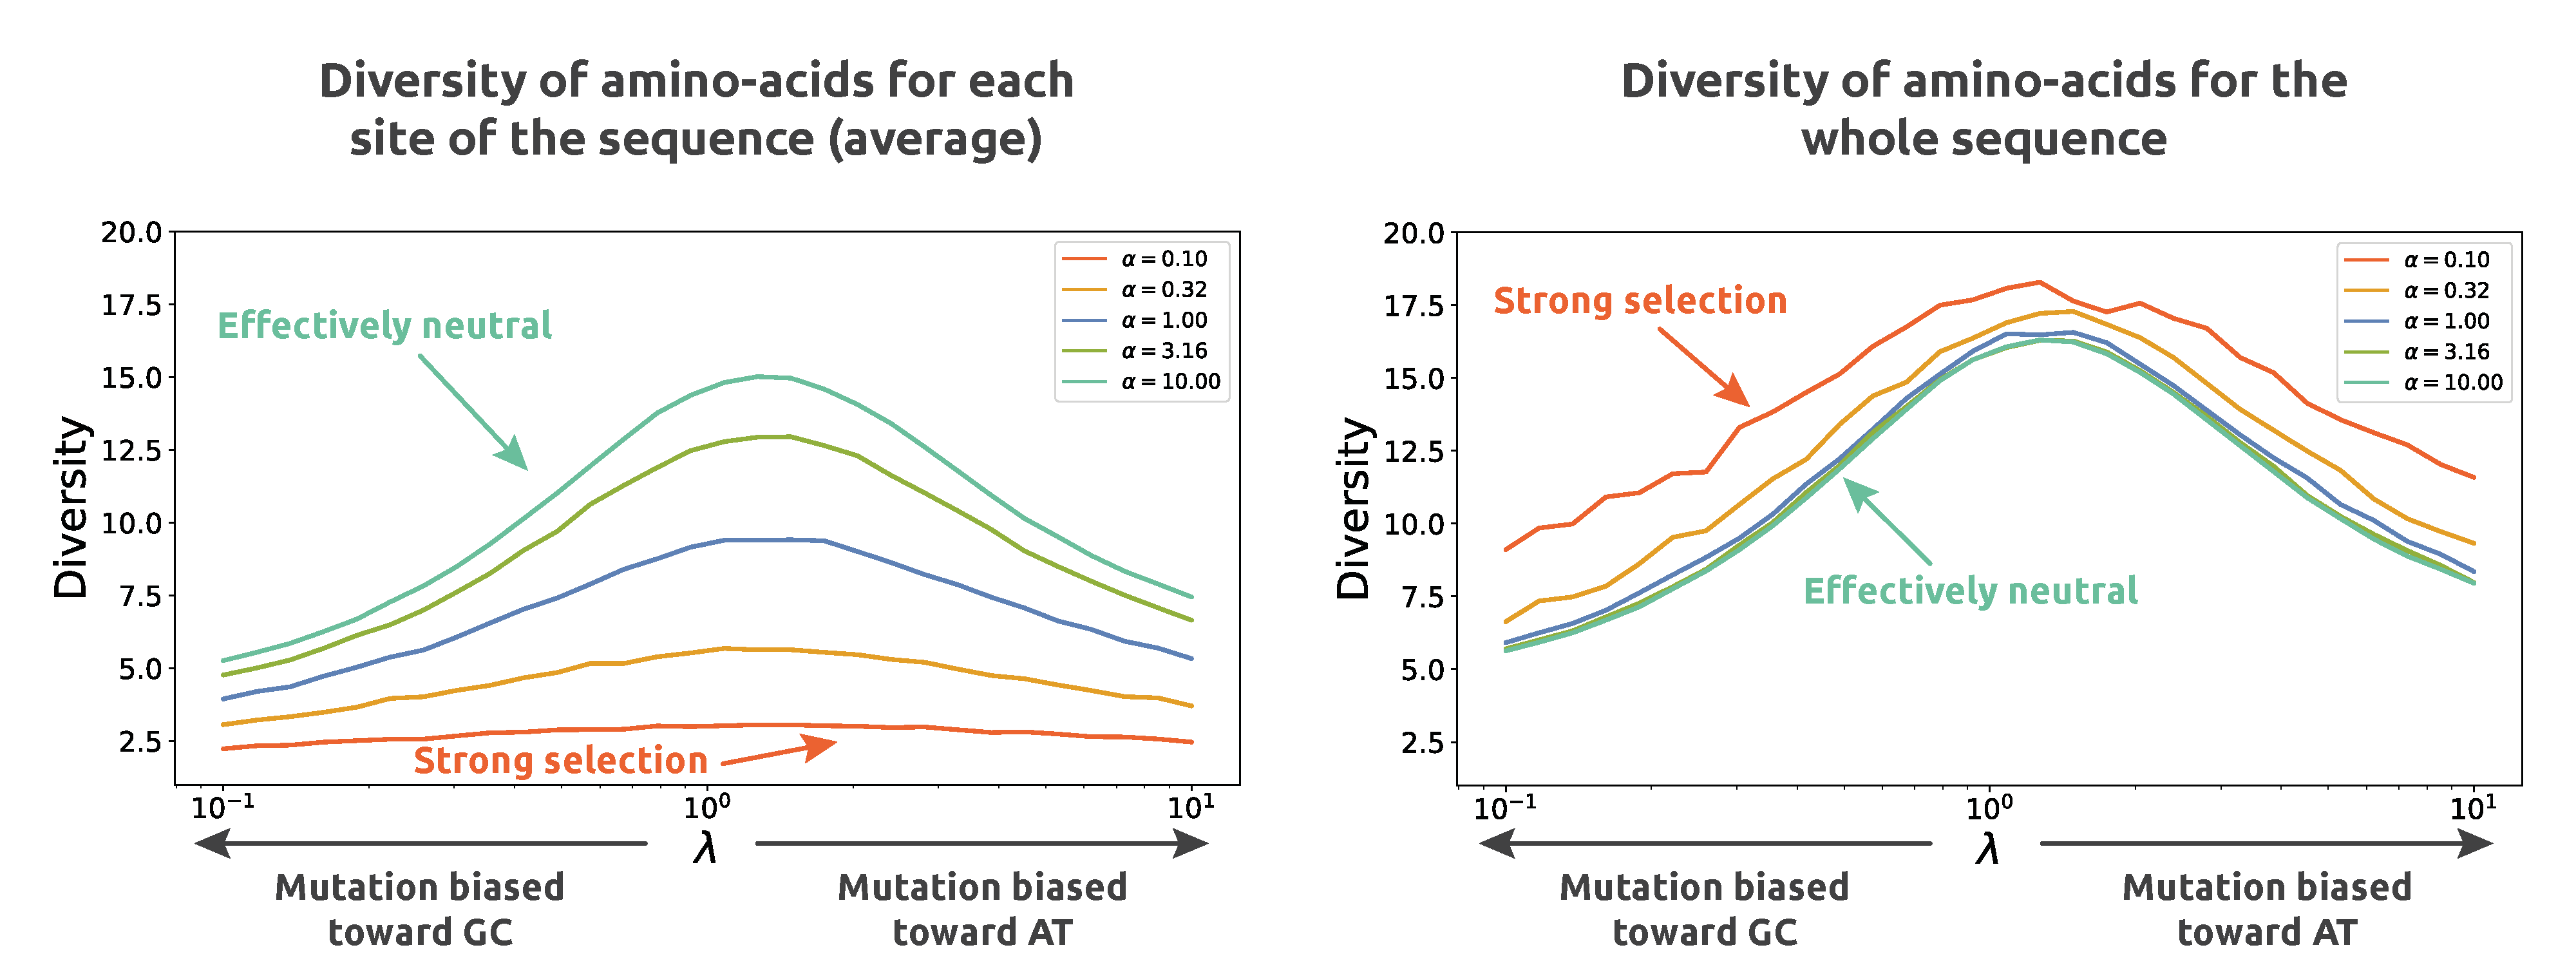
\includegraphics[width=\textwidth] {diversity-aa}
    \caption[Diversity of amino acids]{
    Diversity of the amino-acid frequencies is quantified as the exponential of Shannon's entropy in the vertical axis, either as site-specific diversity in the left panel or as sequence diversity in the right panel.
    Sequence diversity is higher than site-specific diversity, because at any given site only a small number of amino acids are actually permissible.
    From a selective perspective, site-specific diversity decreases with stringency of selection (decreasing $\alpha$ represented by 5 different solid lines) because at given site only a few amino acids are permitted.
    Conversely, because site-specific fitness profiles are randomly drawn, each site has different permitted amino acid, increasing the sequence diversity as the stringency of selection increases.
    From a mutational perspective, diversity decreases with increased mutational bias toward either toward AT or GC ($\lambda$ in horizontal axis).
    This effect is explained by the high frequency of amino acids containing nucleotides favoured by the underlying mutational bias.
    Finally, under stringent selection, diversity is less sensitive to the underlying mutational bias.}
    \label{fig:mut-bias-diversity-aa}
\end{figure}

%Evolutionary rate, which measures the rate at which mutations at individual sites arise and go to fixation, is governed by the amino acid distribution of individual sites, not the average distribution over a broad class of sites.
%The substitution rate (e.g., Grishin, Wolf \& Koonin, 2000).
%These two measures of evolutionary variability are considered to be essentially equivalent~\citep{Halpern1998}, though they are differently influenced by the mutational process~\citep{Santos2018}.

However, the diversity obtained from the observed alignment is biased by phylogenetic inertia, since the sequences are not independent of each others but related together by a specie tree.
In addition, the observed diversity does not relate directly to the fixation probability of proposed mutations.
Instead, the mean scaled fixation probability of non-synonymous mutations ($\avgpfix$), which measures the rate at which mutations arise and go to fixation relatively to neutral mutation, is an aggregate parameter measuring the overall strength of selection throughout the process.
Moreover, $\avgpfix$ can be quantified from the substitutions recorded along the simulation (see section~\ref{subsec:fixation-bias}).
This parameter identifies with the ratio of non-synonymous over synonymous substitution rates, often called $\omega$ or $\dnds$~\citep{Spielman2015, DosReis2015, Jones2016}.
As expected, $\avgpfix$ is always lower than $1$ for simulation under a time-independent fitness landscape~\citep{Spielman2015}, and depends strongly on the stringency of selection ($\alpha$) as depicted in left panel of figure~\ref{fig:mut-bias-omega-WS}.
However, $\avgpfix$ depends weakly on the mutational bias ($\lambda$), contrarily the diversity highly dependent on $\lambda$.

This proxy of selection concerns all non-synonymous mutations, but we can consider the mean scaled fixation probability only for the subset of non-synonymous mutations from weak nucleotides (A or T) to strong nucleotides (G or C), called $\avgpfix_{\ATtoGC}$.
In this context, $\avgpfix_{\ATtoGC}$) increases in response to stronger mutational bias toward AT (i.e. with increasing $\lambda$), which had pushed codon containing favoured nucleotides toward less fit amino acid, as seen in the right panel of figure~\ref{fig:mut-bias-omega-WS}.
This distortion of selective effects toward GC is stronger with increased stringency of selection (i.e. with decreasing $\alpha$) .
Altogether, fixation probabilities are opposed to mutational bias, where the sequence is at an equilibrium point between these two forces.

\begin{figure}[htbp]
    \centering
    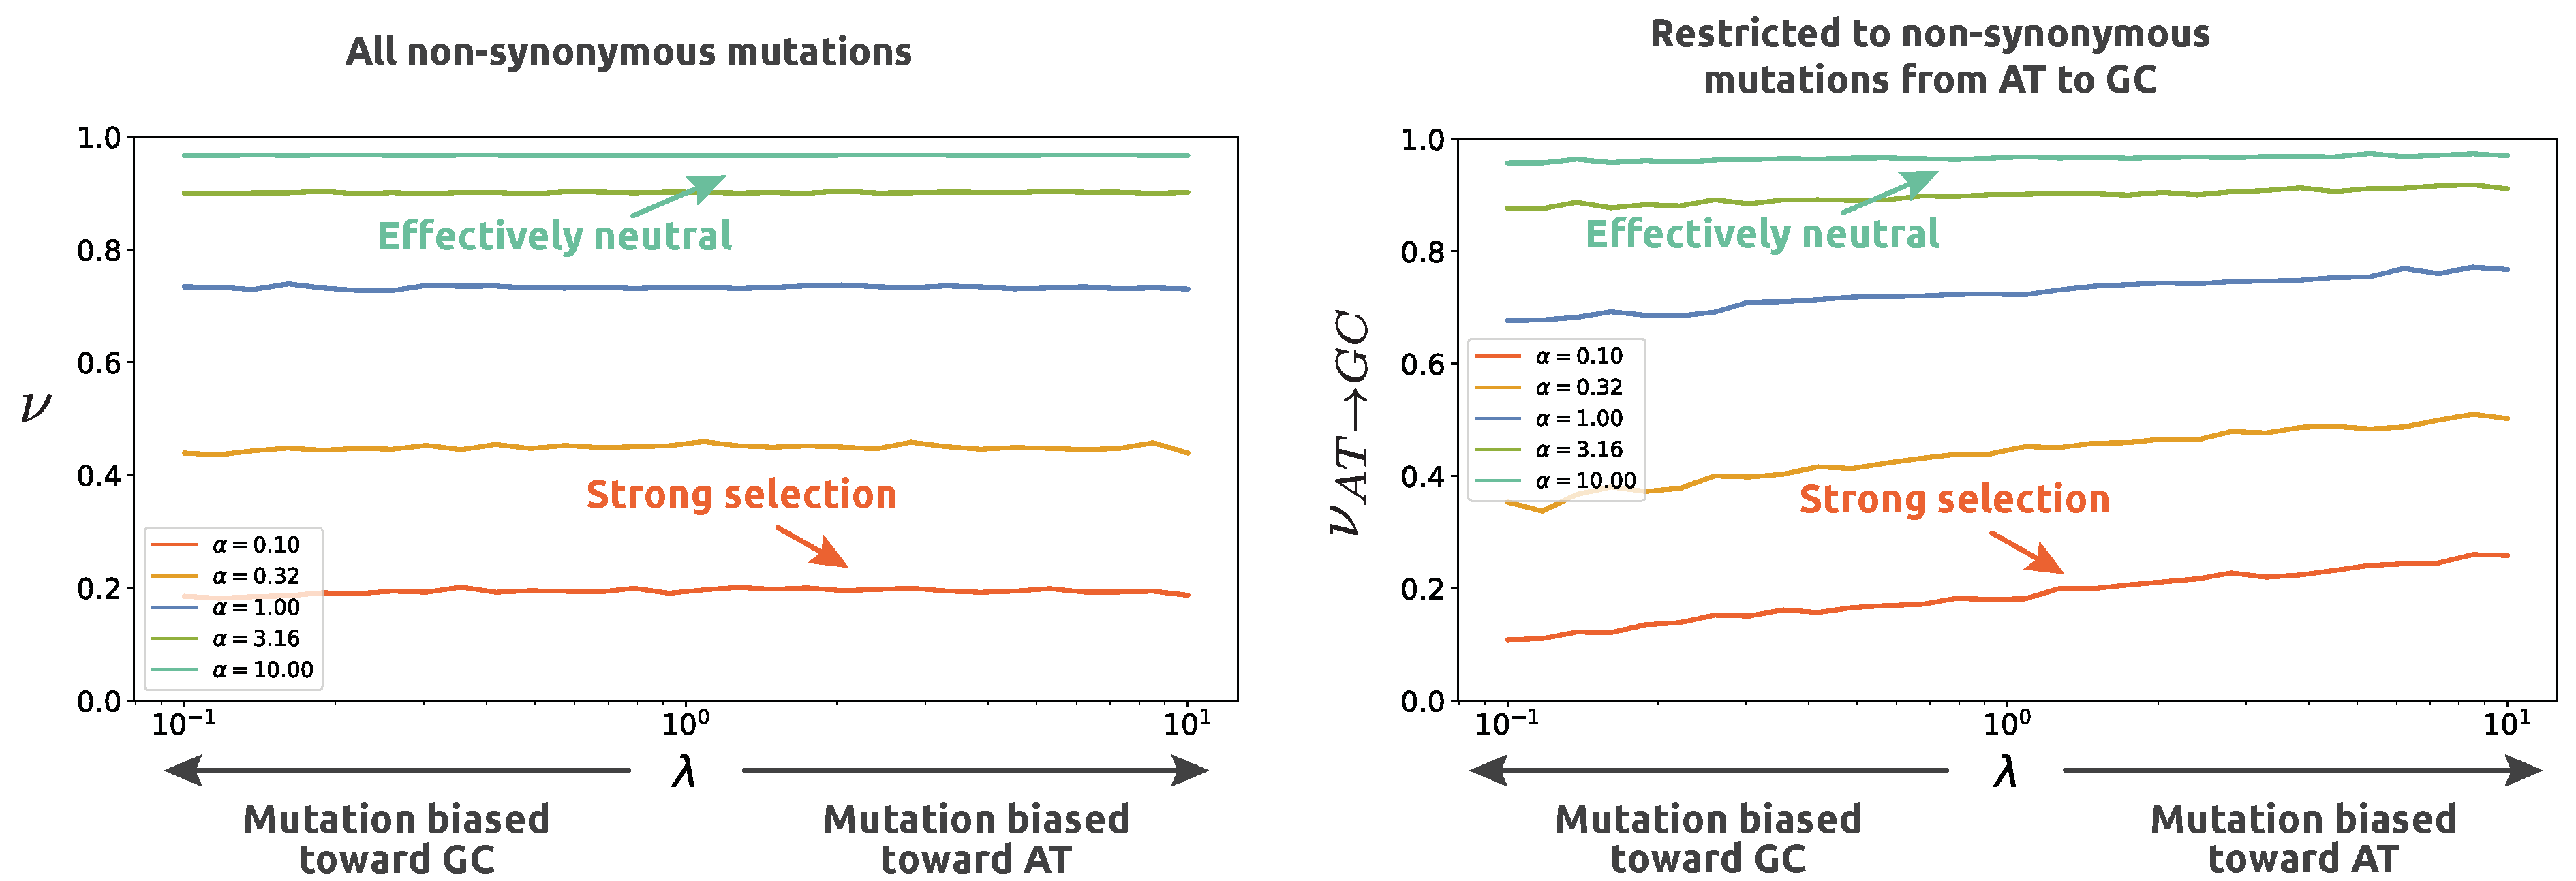
\includegraphics[width=\textwidth] {omega-AT-to-GC}
    \caption[Mean scaled fixation probability as a function of the parameters]{
    Mean scaled fixation probability ($\avgpfix$) in vertical axis as a function of mutational bias ($\lambda$) in the horizontal axis, for different stringency of selection ($\alpha$) in coloured solid lines.
    In the left panel, expectedly, $\avgpfix$ decrease with increased strength of selection (i.e. with decreasing $\alpha$).
    However, $\avgpfix$ is relatively unaffected by the mutational bias ($\lambda$).
    In the right panel, the mean scaled fixation probability of non-synonymous mutations is restricted to mutations from weak nucleotides (AT) to strong nucleotides (GC), called $\avgpfix_{\ATtoGC}$, represented in the vertical axis.
    A mutational process biased towards AT leads to an increased fixation probability toward GG, in the opposite direction.
    More generally, mutation bias is balanced by selection, where this effect increases with the stringency of selection.
    }
    \label{fig:mut-bias-omega-WS}
\end{figure}

\subsection{Parameter inference on simulated data}
\label{subsec:parameter-inference-on-simulated-data}

From an alignment of protein-coding \acrshort{DNA} sequences, without knowing the specific history of substitutions, estimates obtained with models of inference can approximate the mutational bias ($\lambda$) and the mean scaled fixation probability ($\avgpfix$).
Once the model is fitted to the data, the estimated parameters ($\widehat{\lambda}$, $\widehat{\avgpfix}$) can be compared to the known value of the simulation, as shown in figure~\ref{fig:mut-bias-pipeline}.

Practically, the likelihood of the data is computed from the tree topology and the instantaneous rates between codons, known as the 61x61 codon substitution matrix ($\Submatrix$).
Here we developed two models of inference, differing only by their parametrization of the codon matrix $\Submatrix$, considered homogeneous along the sequence (not site-specific).
Two models of inference are proposed, the first is based on \citet{Muse1994} formalism, and the second is based on a tensor of mean scaled fixation probabilities introduced in this study.

\begin{figure}[htbp]
    \centering
    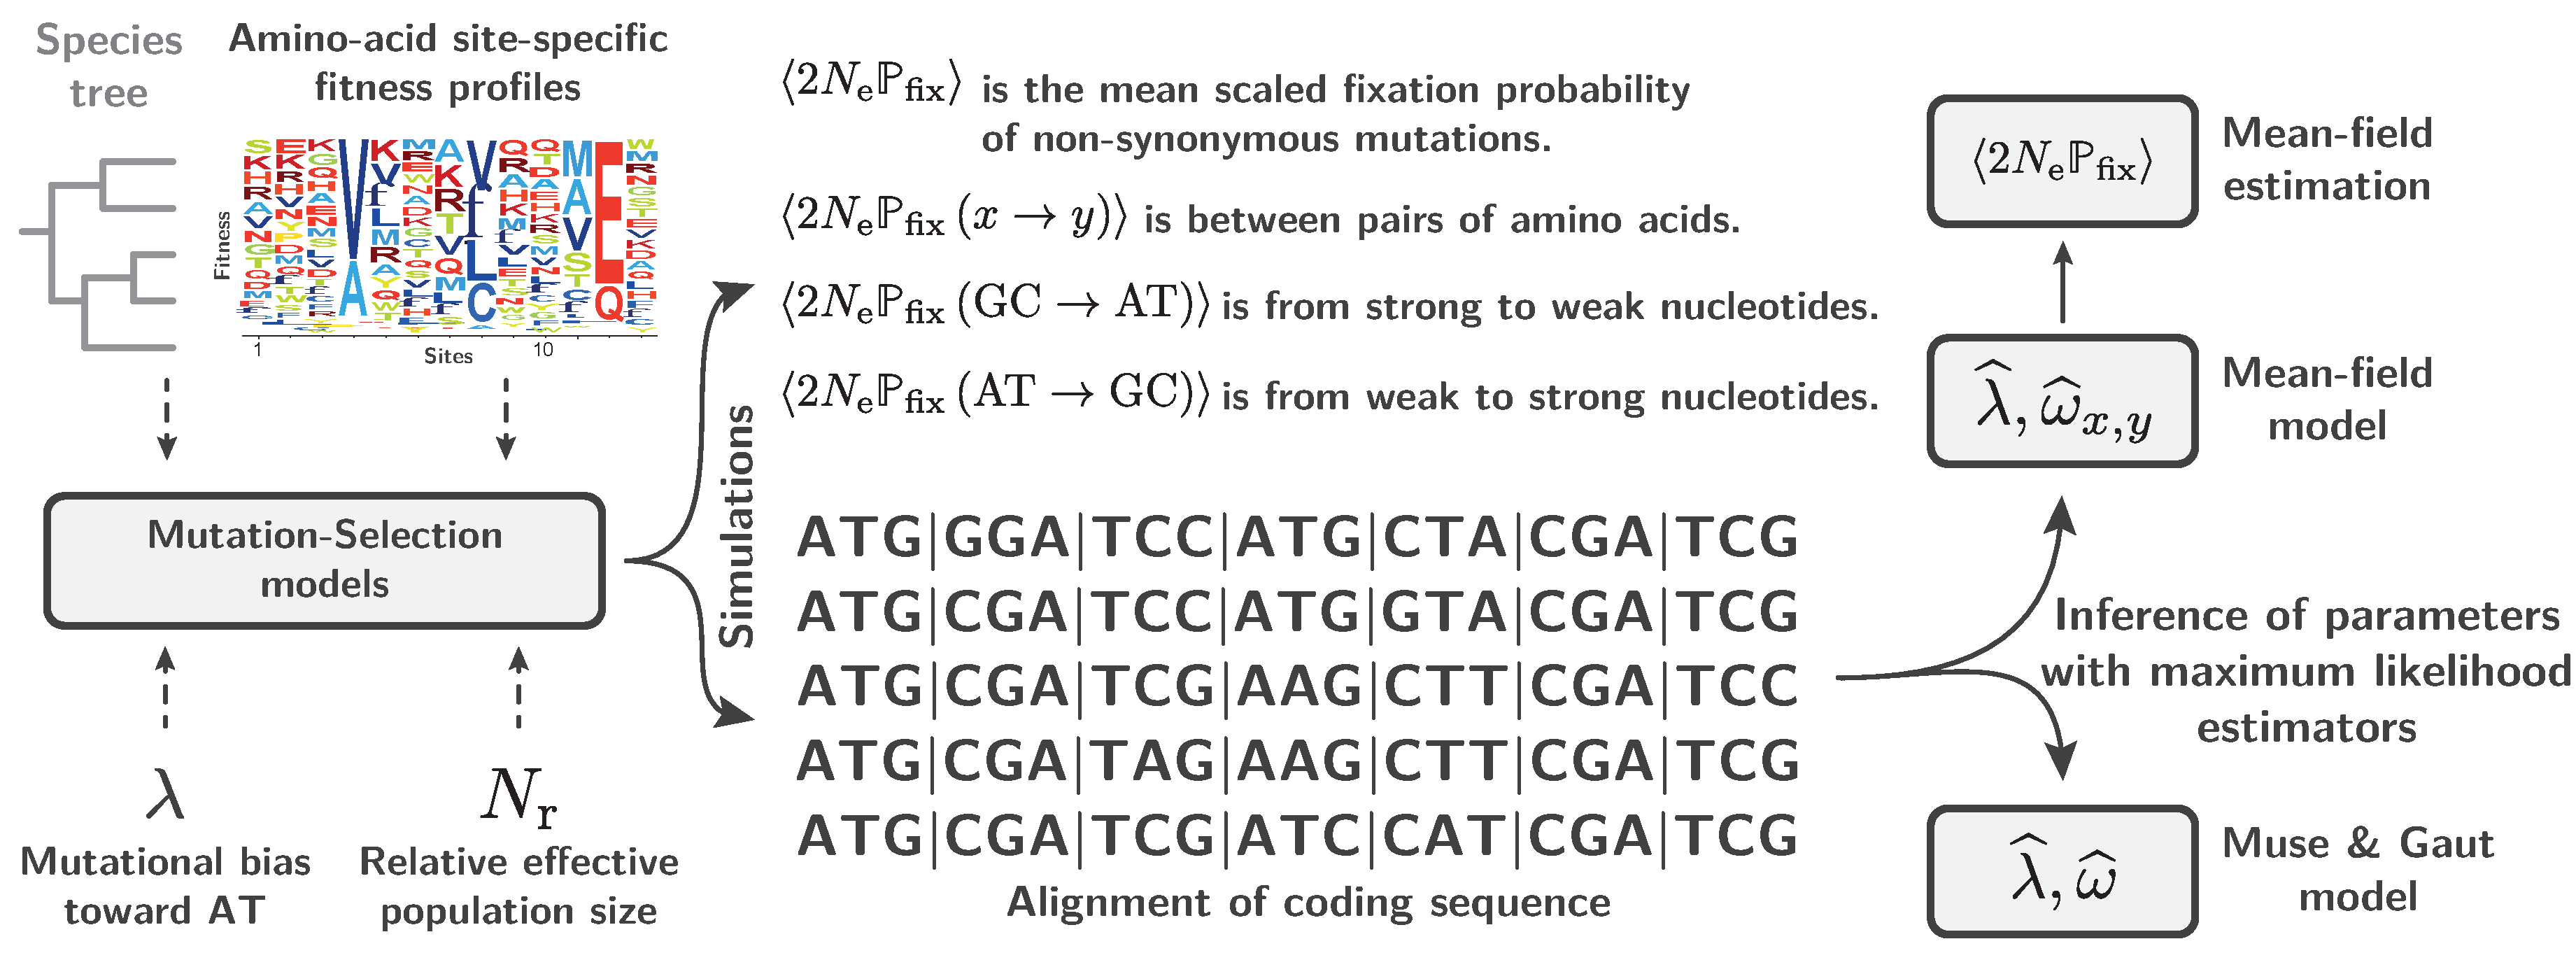
\includegraphics[width=\textwidth, page=1] {pipeline}
    \caption[Inferred value compared to known value]{
    Inferred value ($\widehat{\lambda}$, $\widehat{\avgpfix}$) compared to underlying value ($\lambda$, $\avgpfix$) of the simulation.
    The different parameterization of the inference model can result in different estimates of mutational bias ($\widehat{\lambda}$) and mean scaled fixation probability ($\widehat{\avgpfix}$).
    The main goal is to derive model of inference that can reliably estimate these parameters.
    Two models of inference are proposed, the first is based on Muse \& Gaut formalism, and the second based on a tensor of mean scaled fixation probabilities.}
    \label{fig:mut-bias-pipeline}
\end{figure}

\subsubsection{\texorpdfstring{$\omega$}{ω} as a scalar with Muse \& Gaut formalism}
At the level of nucleotides, the mutation rate is defined entirely by a generalized time-reversible nucleotide mutation rate matrix $\Mutmatrix$, which is a function of the nucleotide frequencies $\Mutequi$ and the symmetric exchangeability rates $\Exchan$~\citep{Tavare1986}:
\begin{equation}
    \mutmatrix_{a, b} = \exchan_{a,b}\mutequi_b
\end{equation}
At the level of codon, the substitution rate between the source ($\ci$) and target codon ($\cj$) depends on the underlying nucleotide change between ($\nucitoj$) and whether or not the change is non-synonymous.
Altogether, the substitution rates between codons $\submatrix_{\itoj}$, formalized by \citet{Muse1994} are function of the mutation matrix $\Mutmatrix(\Mutequi, \Exchan)$, a single parameter of selective strength $\omega$, and the genetic code as:
\begin{equation}
    \begin{dcases}
        \submatrix_{\itoj} & = 0 \text{ if codons $\ci$ and $\cj$ are more than one mutation away,} \\
        \submatrix_{\itoj} & = \mutmatrix_{\nucitoj} \text{ if codons $\ci$ and $\cj$ are synonymous,} \\
        \submatrix_{\itoj} & = \omega \mutmatrix_{\nucitoj} \text{ if codons $\ci$ and $\cj$ are non-synonymous}.
    \end{dcases}
    \label{eq:codon-muse-gaut}
\end{equation}

Phenomenological codon models are not designed to tease out mutational bias, but firstly to estimate the global strength of selection ($\omega$).
From the maximum likelihood estimates of the \acrshort{GTR} mutation matrix ($\widehat{\Mutmatrix}$), we can estimate of the mutational bias toward $\text{AT}$ as $\widehat{\lambda}_{\text{MG}} = (\widehat{\mutequi_A} +\widehat{\mutequi_T}) /(\widehat{\mutequi_G} +\widehat{\mutequi_C}) $.
As shown in the left panel of figure~\ref{fig:mut-bias-inference}, estimate of the mutational bias is halfway between observed bias of the alignment and the true value used during the simulation.
As a result, this model cannot reliably infer the mutational bias, and is doing a compromise between estimating the selection coefficients and mutational bias.
We can also estimate the parameter ${\widehat{\omega}_{\text{MG}}}$, which is close to the underlying mean scaled fixation probability $\avgpfix$ computed during the simulation, with a precision of 98.2\%.

\subsubsection{\texorpdfstring{$\omega$}{ω} as a tensor with mean-field derivation}

Alternatively, gene-wide parameters of fixation should attempt to capture and aggregate site-specific parameterization of evolution.
As a result, projecting site-specific processes into a gene-wise process can be seen as a mean-field approximation, accounting for mean scaled fixation probability between amino acids, even though done at the level of the gene.

Because selection between codons reduces to selection between pairs of amino-acids, the mean-field approximation is parameterized by mean scaled fixation probability between all pairs of amino acids, denoted $\omega_{\aaSource, \aaTarget}$.
For $20$ amino acids, the total number of pairs of amino acid is $190$, hence $380$ parameters by counting in both directions.
However, because of the structure of the genetic code, they are $75$ pairs that are one nucleotide away, since some amino acids are not directly accessible through a single non-synonymous mutation.
As a result, the number of parameters necessary to determine all mean scaled fixation probability ($\omega_{\aaSource, \aaTarget}$) in both directions is $150$.
However, under the assumption of a reversible process, the number of parameters can be reduced to $75$ parameters of exchangeabilities ($\beta_{\aaSource, \aaTarget}$) and $20$ parameters of stationary distribution ($\epsilon_{\aaSource}$).
\begin{align}
    \omega_{\aaSource, \aaTarget} = \epsilon_{\aaTarget} \beta_{\aaSource, \aaTarget}\text{, where } \beta_{\aaSource, \aaTarget} = \beta_{\aaTarget, \aaSource}.
\end{align}

Under projected mutation-selection model, the substitution rates between codons $\submatrix_{\itoj}$ are defined from a GTR mutation matrix $\Mutmatrix(\Mutequi, \Exchan)$, the selection coefficients $\bm{\omega}(\bm{\beta}, \bm{\epsilon})$ and the genetic code:
\begin{equation}
    \begin{dcases}
        \submatrix_{\itoj} & = 0 \text{ if codons $\ci$ and $\cj$ are non neighbors}, \\
        \submatrix_{\itoj} & = \mutmatrix_{\nucitoj} \text{ if codons $\ci$ and $\cj$ are synonymous,}, \\
        \submatrix_{\itoj} & = \mutmatrix_{\nucitoj} \omega_{\aai, \aaj} \text{ if codons $\ci$ and $\cj$ are non-synonymous},
    \end{dcases}
    \label{eq:codon-mean-field}
\end{equation}
where $\aai$ is the amino acid encoded by codons $\ci$.

From the maximum likelihood estimates of the \acrshort{GTR} mutation matrix ($\widehat{\Mutmatrix}$), we can estimate the mutational bias $\left({\widehat{\lambda}_{\text{MF}}} \right)$ as previously.
As shown in the right panel of figure~\ref{fig:mut-bias-inference}, this model can tease out observed $\atgc$ of the alignment and the underlying mutational bias.
We can also estimate the mean scaled fixation probability of non-synonymous mutations $\widehat{\avgpfix}_{\text{MF}}$ (see section~\ref{sec:mut-bias-mean-field-omega}) which is a compound parameter of $\Mutmatrix(\Mutequi, \Exchan)$ and $\bm{\omega}$.
Under this model, $\widehat{\avgpfix}_{\text{MF}}$ is close to the $\avgpfix$ computed during the simulation, with a precision of 97.0\%.

\begin{figure}[htbp]
    \centering
    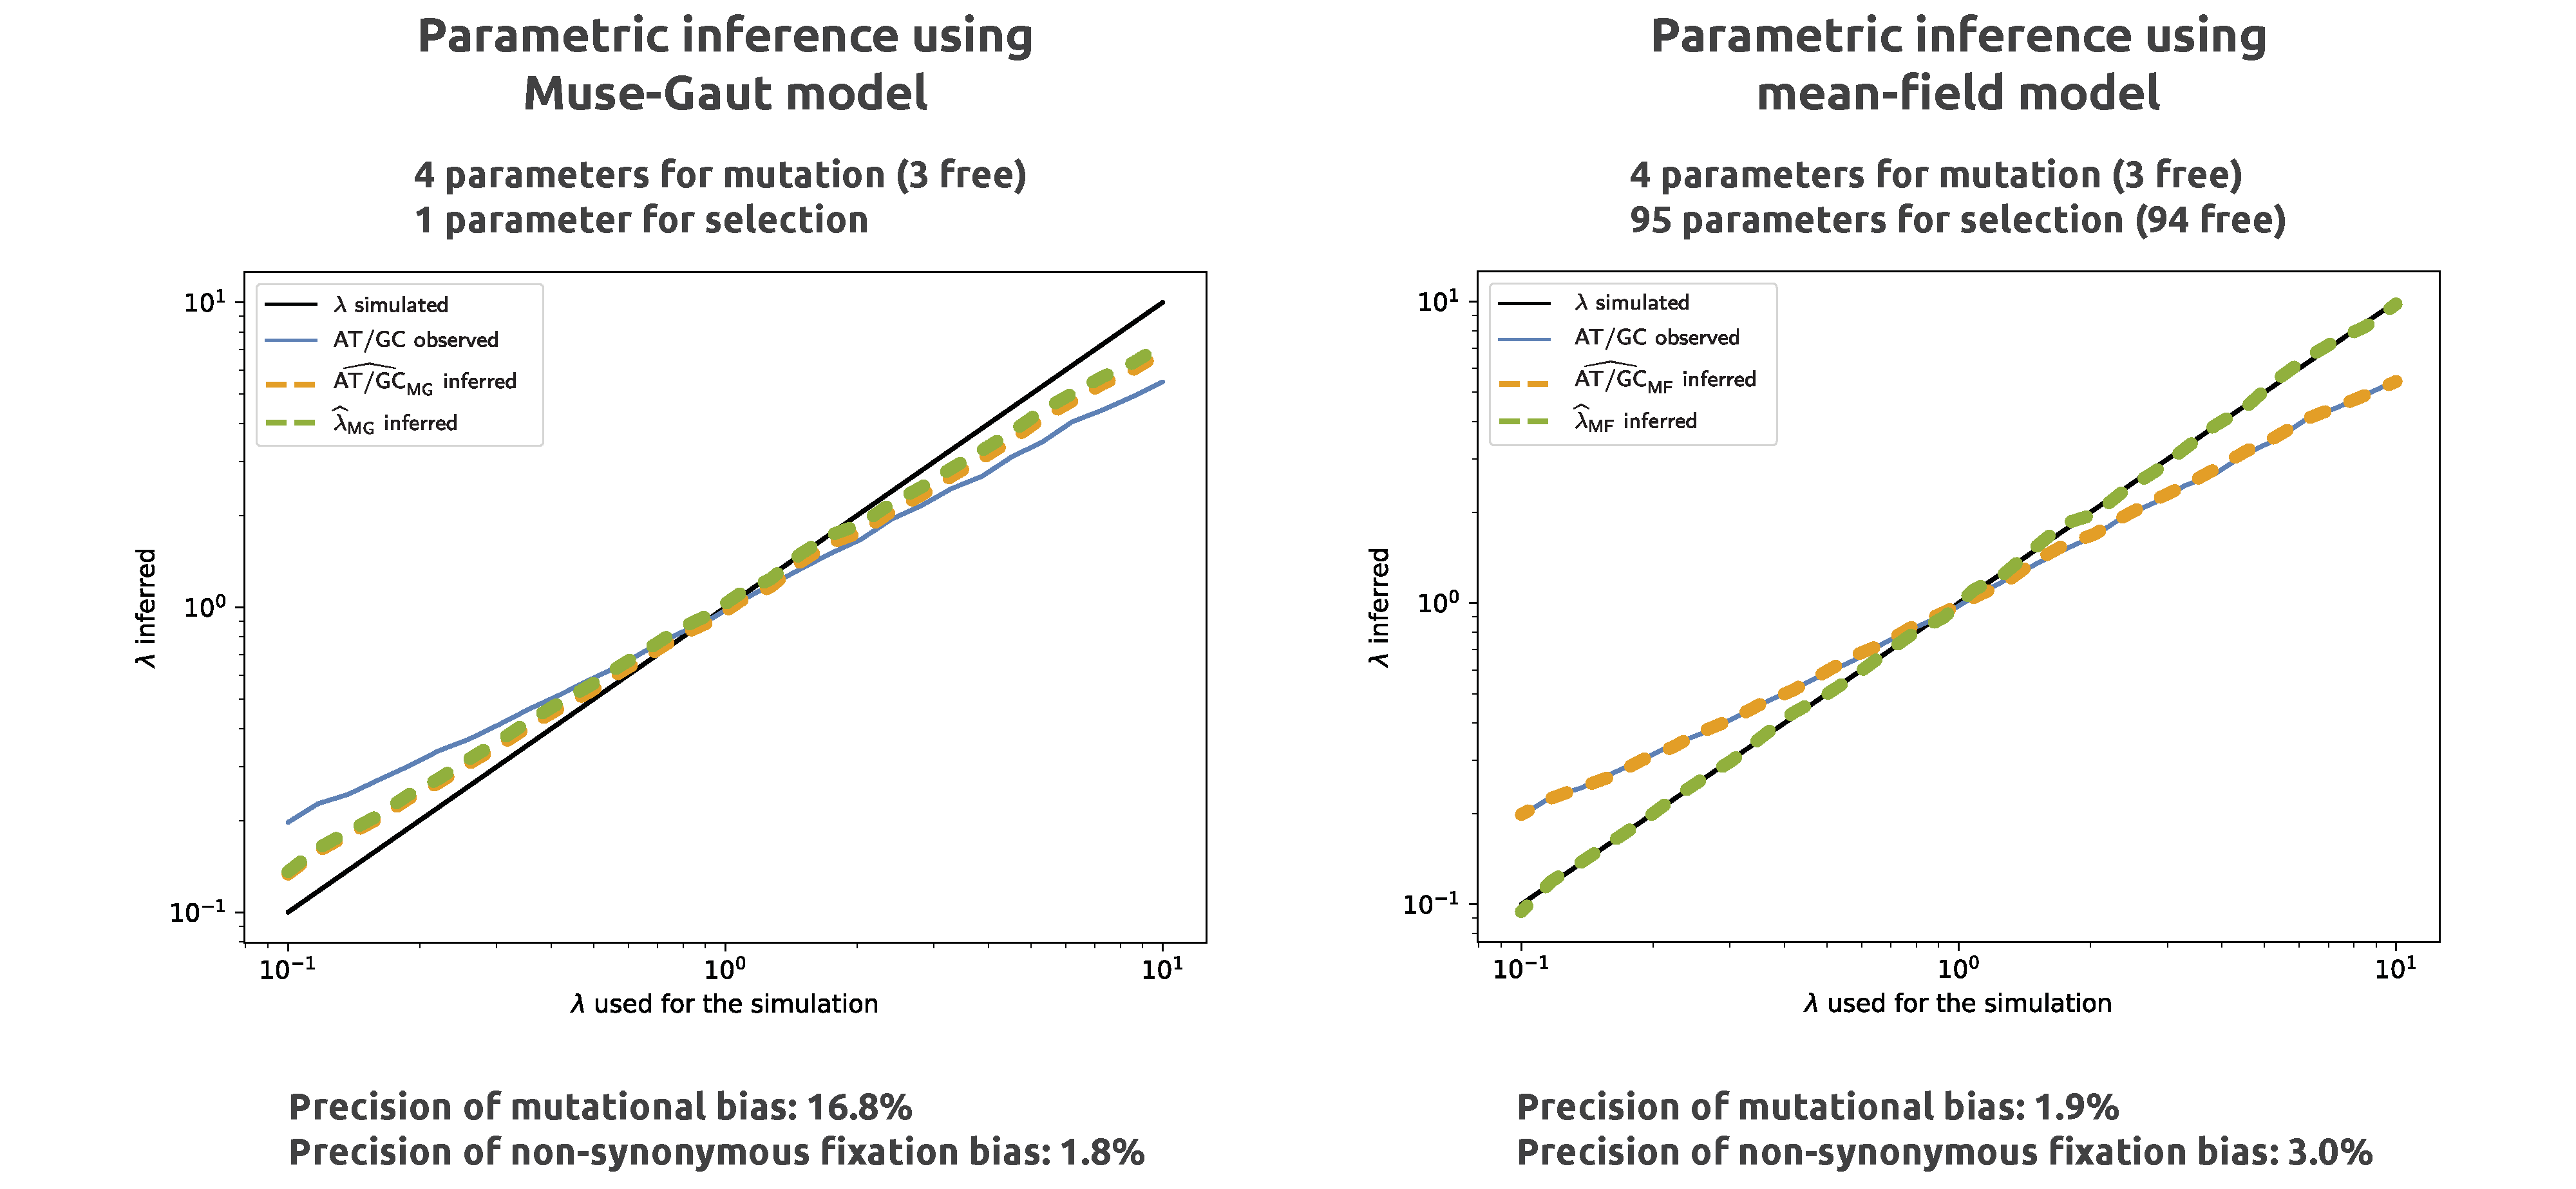
\includegraphics[width=\textwidth] {Simulation-vs-Inference}
    \caption[Estimation of mutationanl bias]{
    Different proxies of estimated mutational bias in the vertical axis are represented as a function of the underlying mutational bias ($\lambda$) of the simulation in the horizontal axis.
    Mutational bias can be estimated directly from the observed nucleotide frequencies in the alignment ($\atgc$ in blue solid line), similarly to figure~\ref{fig:mut-bias-AT-GC-obs}, which is skewed by selection and always less extreme than the underlying mutational bias.
    The robustness of mutational bias estimation of two different inference models are shown.
    Selection is modelled as a single $\omega$ parameters in the Muse \& Gaut formalism in the left panel, while selection is modelled as a tensor of $\omega$ parameters in different directions using a mean-field approximation in the right panel.
    In both panels, the true value of the mutational bias is represent in black solid line.
    The estimated mutational bias $\widehat{\omega}_{\text{MG}}$ (in yellow dotted line) in the Muse \& Gaut formalism is between the true value and the observed $\atgc$.
    Conversely, estimated mutational bias $\widehat{\omega}_{\text{MG}}$ (in yellow dotted line) in the mean-field approximation equal to the underlying value.
    Moreover, the expected $\widehat{\atgc}$ from the parameter of the model fits the observed value in the mean-field approximation, while being skewed in the Muse \& Gaut formalism.
    Altogether, the mean-field approximation can tease apart mutation and selection, while the Muse \& Gaut formalism has to reach a compromise between observed $\atgc$ and underlying mutational bias.
    }
    \label{fig:mut-bias-inference}
\end{figure}

\subsection{Estimation of empirical sequence data}
\label{subsec:estimation-of-empirical-sequence-data}

The two models of inference (classical Muse \& Gaut and mean-field) can be applied to empirical alignment.
Also, in empirical data we observed that the mean scaled fixation probability between weak and strong nucleotide is not equal, and is opposite of the nucleotide bias (see table~\ref{tab:mut-bias-estimation}).

\begin{table}[htbp]
    \centering
    \noindent\adjustbox{max width=\textwidth}{%
    \begin{tabu}{|c||c|c|}
        \hline
        \textbf{Estimated parameter} & Nucleoprotein & Lactamase \\
        \hline \textbf{$\atgc$ of the alignment} & 1.15 & 0.79 \\
        \hline \textbf{Muse-Gaut mutational bias $\left({\widehat{\lambda}_{\text{MG}}} \right)$ } & 1.39 & 0.85 \\
        \hline \textbf{Mean-field mutational bias $\left({\widehat{\lambda}_{\text{MF}}} \right)$} & 1.64 & 0.68 \\
        \hline \textbf{Mean-field fixation ratio from AT to GC $\left(\widehat{\avgpfix}_{\ATtoGC}\right)$} & 0.14 & 0.31 \\
        \hline \textbf{Mean-field fixation ratio from GC to AT $\left(\widehat{\avgpfix}_{\textbf{GC} \rightarrow \textbf{AT}}\right)$} & 0.10 & 0.44 \\
        \hline
    \end{tabu}}
    \caption[Estimated parameters]{
    Estimated parameters
    Nucleoprotein alignment of 498 amino acids available for 180 species (left column).
    Lactamase alignment of 263 amino acids available for 85 species (right column).
    }
    \label{tab:mut-bias-estimation}
\end{table}


\section{Discussion}\label{sec:discussion}

The observed composition of \acrshort{DNA} sequences is the result of the interplay between mutation and selection, such that the observed mutational bias in the alignment is different to the underlying mutational bias.
In protein-coding \acrshort{DNA} sequences, the nucleic composition result in the subtle interplay between mutation at the nucleic level and selection at the protein level.
For example, mutational bias toward AT is balanced by selection in the opposite direction toward GC, potentially a confounding effect with \acrshort{gBGC}.

Unfortunately, parametric codon models developed to estimate the rate of evolution on amino acids use the observed mutational bias at the protein level, discarding the effect of selection.
We show that even if the mutational process is misspecified, parametric codon models are able to estimate reliably the rate of evolution acting on amino acids.
However, such parametric codon models are inherently misspecified to untangle mutation and selection, and they don't estimate the mutational process reliably.
Reliable inference of mutational bias thus requires to model selection in different directions.

In this work we seek to find the simplest parametric codon model able to correctly tease apart mutation rates on one hand, and net mean fixation probabilities without having to explicitly model the underlying fitness landscape.
In order to derive a codon model along those lines, our strategy is to first assume a true site-specific evolutionary process, following the mutation-selection formalism.
For the sake of simplicity and illustration, we assume a site-specific, time-independent fitness landscape.
Then, we derive the mean substitution process implied across all sites by this site-specific mechanistic model.
This mean-field $61$x$61$ substitution matrix is expressed in terms of mutation rates and average fixation probabilities.
Finally, we identify average fixation probabilities appearing in this expression with the $\omega$ tensor we are looking for.
What we show is that we should in fact invoke as many distinct $\omega$ parameters as there are pairs of amino acids that are nearest neighbours in the genetic code.
There are reversibility conditions, reducing the dimensionality and allowing for a GTR-like parameterization of this tensor ($95$ parameters for selection).

Inferring parameters on simulated alignments, we show that the model correctly estimates the mutation rates.
Our mean-field parametric model use gene-wise parameters of mean scaled fixation probabilities, and even though the underlying selective landscape is site-specific, such approximation can nonetheless be used to disentangle mutation and selection.

This work points to a fundamental behavior of molecular sequences, namely that they are not optimized but are the result of an equilibrium between forces.
Fixation bias or selective effects can be a response to another underlying mechanism, in this case mutational bias.

As an example, observed selective effect toward GC, mimicking biased gene conversion toward GC (\acrshort{gBGC}) can be a byproduct of an underlying mutational bias toward AT.
Our observations and modelling principles offers tools to better understand how mutation-mutation will work together with biased gene conversion (\acrshort{gBGC}), and therefore also yields better understanding of how \acrshort{gBGC} will impact both nucleotide composition and $\dnds$.

This study demonstrates that phenomenological models derived out of mechanistic models are more compact, and in certain cases are sufficient to extract relevant parameters.
Models of inference are classified broadly into phenomenological and mechanistic~\citep{Rodrigue2010a}.
Mechanistic models dissect the detailed causal chain of events responsible for each substitution event and then use this to construct a detailed model from first principles.
By doing this, they relate structural, population genetics and ecological parameters to the likelihood function (see chapter~\ref{chap:MutSelDrift}).
As such, mechanistic inference models are suitable to construct an integrative framework, for example relating the signal available in molecular sequences to structural parameters, expression level across genes and varying effective population size across lineages.
Once such models have been fitted to empirical data, the estimated parameters can then be confronted with independent estimations, which allow one to robustly test the model since independent estimates of biological and ecological parameters should of course be congruent~\citep{Dasmeh2014}.
However mechanistic models are computationally very intensive, to a point where they can reach the current limits in available computing power.
Apart from this physical limit of resource available, the use of computing resources bears ecological consequences on environmental degradation and $C0_2$.
Moreover, increased complexity of the models bears another consequence: the liability of the code and software decreases, compromising the reproducibility of the results obtained with such models.
For these reasons (and primarily the computational limitations), mechanistic models tend to make a number of strong simplifying assumptions (such as no epistasis), which can have detrimental effects on the robustness of the inference (see chapter~\ref{chap:MutSelDrift}).
In contrast, phenomenological models are formulated in terms of aggregate parameters, capturing the average rate of synonymous or non-synonymous substitutions, or their ratio.
Their aim is to determine the statistical distribution of these aggregate quantities across the tree, across genes, or across sites, but without deriving them from first principles.
Compared to mechanistic models, they are computationally much more efficient.
On the other hand, they do not give direct access to the population-genetic parameters.
This raises the question of how to benefit from the advantages of the two approaches.
Observations and experiments done throughout this thesis led me to crystallize the conception that models of inference should be mechanistic in essence, in the sense that they should be parameterized by variables that are derived from first principles.
But should be phenomenological in practice, in the sense that these variables should nevertheless be aggregate parameters.


\section{Materials \& Methods}

\subsection{Simulation model}
\label{sec:mut-bias-simu}
We seek to simulate the evolution of protein-coding sequences along a specie tree.
Starting with one sequence at the root of the tree, the sequences evolves independently along the different branches of the tree by point substitutions, until they reach the leaves.
At the end of the simulation, we get one sequence for each leaf of the tree, meaning one sequence per specie.
Such evolutionary process is an idealized version of the reality, in the sense that the whole heterogeneity of sequences in the population is discarded, with only one sequence representing the whole population.
For a protein-coding \acrshort{DNA} sequence, a substitution is modelled as the product of mutation at the nucleotide level, and selection at the amino-acid level.

On one hand, the mutation rate between nucleotides as assumed to be shared by all sites of the sequences.
On the other hand, the selection for amino acids is assumed to be varying along the sequences.
During the simulation, from a given sequence, the substitution rate toward all possible mutant (one nucleotide change) is computed and the next substitution at the waiting time until such event is obtained by Gillespie's algorithm~\citep{Gillespie1977}.

\subsection{Mutational bias at the nucleotide level}
\label{sec:mut-bias-mut-matrix}
The mutation rate between nucleotides is always proportional to $\mu$.
Moreover, mutations from any nucleotide to another weak nucleotide is increased by the factor $\lambda$ compared with mutations to another strong nucleotide.
The rate at which a nucleotide doesn't change is given such as the sum of all rates is zero.
The mutation rate matrix is:
\begin{equation}
    \label{nucMatrix}
    \Mutmatrix =
    \begin{blockarray}{ccccc}
        & A & C & G & T \\
        \begin{block}{c(cccc)}
            A & {-\mu(2 + \lambda)} & {\mu} & {\mu} & {\mu \lambda} \\
            C & {\mu \lambda} & {-\mu(1 + 2\lambda)} & {\mu} & {\mu \lambda} \\
            G & {\mu \lambda} & {\mu} & {-\mu(1 + 2\lambda)} & {\mu \lambda} \\
            T & {\mu \lambda} & {\mu} & {\mu} & {-\mu(2 + \lambda)} \\
        \end{block}
    \end{blockarray}
\end{equation}
The stationary distribution $ \Subequi$ must be annihilated by the mutation matrix $\Mutmatrix$, which gives the stationary distribution:
\begin{align}
    \Mutequi \Mutmatrix & = 0, \\
    \iff \Mutequi & = \left( \dfrac{\lambda}{2+2\lambda}, \dfrac{1}{2+2\lambda}, \dfrac{1}{2+2\lambda}, \dfrac{\lambda}{2+2\lambda} \right).
    \label{nucStationarity}
\end{align}
The process is reversible and fulfils detailed balance conditions for any pair of different nucleotides:
\begin{align}
    \mutequi_a \mutmatrix_{a, b} =\mutequi_b \mutmatrix_{b, a}.
    \label{nucMutBalance}
\end{align}
It is important to note that ratio of weak over strong nucleotides frequency at stationarity is equal to $\lambda$:
\begin{align}
    \label{lambda}
    \dfrac{ \mutequi_A + \mutequi_T }{ \mutequi_C + \mutequi_G }
    & = \dfrac{ \lambda ( 2 + 2 \lambda)^{-1} + \lambda ( 2 + 2 \lambda)^{-1}}{ ( 2 + 2 \lambda)^{-1} + ( 2 + 2 \lambda)^{-1}}, \ \text{from eq.~\ref{nucStationarity},}\\
    & = \lambda.
\end{align}

\subsection{Selection at the amino-acid level}
\label{sec:mut-bias-aa-selection}
The substitution rate is considered null if the pair of codons differs by more than one nucleotide.
Otherwise, the mutation rate between a pair of codons is given by the mutation rate of the underlying nucleotides.
We subsequently take into account the selection at the amino-acid level, where each amino acid $\aai$ encoded by codons $\ci$ are given a fitness ($\Fiti$).
By modelling fitness at the amino-acid level, we assume that all codons encoding for one particular amino acid are selectively neutral.
In this modelling framework, the genetic code is of particular importance since the number of codons encoding for a particular amino acid varies greatly.
As an example, tryptophan is encoded by one codon, while leucine is encoded by 6 codons.
Intuitively, this variation makes the mutation bias more pronounced in codons encoding for the same amino acids, since there are more mutations possible that are selectively neutral (i.e synonymous).
On the other hand, the mutation bias is more constrained if the amino acid is encoded by a few codons since there are only a few (or not any) synonymous mutations.

To take into account the heterogeneity of selection between different sites of the protein, we assume that each site $\site$ of the sequence is evolving under a different fitness landscape ($\Fiti\siteexp$).
At one particular site, under a time-independent fitness landscape, the substitution rate between codons is given by the product of the mutation rate and the probability of fixation:
\begin{equation}
    \begin{dcases}
        \submatrix_{\itoj}\siteexp & = 0 \text{ if codons $\ci$ and $\cj$ are more than one mutation away,}\\
        \submatrix_{\itoj}\siteexp & = \mutmatrix_{\nucitoj} \text{ if codons $\ci$ and $\cj$ are synonymous,} \\
        \submatrix_{\itoj}\siteexp & = \mutmatrix_{\nucitoj} \dfrac{\Fitj\siteexp - \Fiti\siteexp}{1 - \e^{\Fiti\siteexp - \Fitj\siteexp} } \text{ if codons $\ci$ and $\cj$ are non-synonymous}.
    \end{dcases}
    \label{eq:codonsubrates}
\end{equation}
At the root the tree, the sequence is obtained by sampling from the equilibrium stationary distribution.
The stationary distribution $\Subequi$ at site $\site$ can be obtained as:
\begin{align}
    \subequi_{\ci}\siteexp & = \mathcal{Z}\siteexp \lambda^{\nbrWeak_{\ci}} \e^{\Fiti\siteexp} \text{ where } \ \mathcal{Z}\siteexp = \left( \sum\limits_{\cj=1}^{61} \lambda^{\nbrWeak_{\cj}} \e^{\Fitj\siteexp} \right)^{-1},
    \label{codonStationarity}
\end{align}
and $\nbrWeak_{\ci}$ is the number of weak nucleotides (A or T) in the codon (between 0 and 3).

Moreover, the substitution process is reversible and fulfils detailed balance conditions at each site $\site$:
\begin{align}
    \subequi_{\ci}\siteexp \submatrix_{\itoj}\siteexp = \subequi_{\cj}\siteexp \submatrix_{\cj, \ci}\siteexp
    \label{codonSubBalance}
\end{align}

The next substitution event, and the time to reach such event is chosen using Gillespie's algorithm~\citep{Gillespie1977}, according to the rates of substitution ($\submatrix_{\itoj}$) between sequences.

\subsection{Diversity of amino-frequencies}
\label{subsec:entropy}

For a site $\site$, the diversity $D\siteexp$ is computed as the exponential of Shannon's entropy from the frequencies of the different amino-acids ($\profile\siteexp$):
\begin{equation}
    D(\profile\siteexp) = \exp \left[ - \sum\limits_{\SetAa} \profile\siteexp_{\aminoacid} \ln \left( \profile\siteexp_{\aminoacid} \right) \right]
    \label{eq:diversity-site-specific}
\end{equation}
The diversity is a measure of the flatness of the fitness profile, with a value of $1$ corresponding to a single peak fitness landscape (i.e. with only one amino acid permissible), and a value of $20$ corresponding to a neutral landscape, where each amino acid has the same fitness.
The diversity can be averaged over all sites as:
\begin{equation}
    \left\langle D(\profile) \right\rangle = \dfrac{1}{\Nsite}\sum\limits_{\Setsite} D(\profile\siteexp)
    \label{eq:diversity-site-specific-avg}
\end{equation}
Otherwise, frequencies of the different amino-acids can first be averaged over all sites:
\begin{equation}
    \left\langle \profile \right\rangle = \dfrac{1}{\Nsite}\sum\limits_{\Setsite} \profile\siteexp
    \label{eq:profile-gene-wise}
\end{equation}
Then the gene-wise diversity is simply:
\begin{equation}
    D \left(  \left\langle \profile \right\rangle \right) = \exp \left[ - \sum\limits_{\SetAa} \left\langle \profile \right\rangle_{\aminoacid} \ln \left( \left\langle \profile \right\rangle_{\aminoacid} \right) \right]
    \label{eq:diversity-gene-wise}
\end{equation}

\subsection{Mean scaled fixation probability}
\label{subsec:fixation-bias}
The sequence at time $t$ is denoted $\Seqi(t)$ and the codon present at site $\site$ is denoted $\Seqi_{\site}(t)$.
For a given sequence, the mean scaled fixation probability of mutations is the ratio :
\begin{align}
    \avgpfix (t) & = \dfrac{ \sum\limits_{\site} \sum\limits_{\cj \in \NonSynNeighbors \left ( \Seqi_{\site}(t) \right)} Q_{\Seqi_{\site}(t) \to \cj}}{ \sum\limits_{\site} \sum\limits_{\left ( \cj \in \Seqi_{\site}(t) \right)} \mu_{\Seqi_{\site}(t) \to \cj}},
\end{align}
where $\setNonSynNeighbors$ is the set of non-synonymous codons neighbors of codon $\ci$ and $\submatrix_{\itoj}\siteexp$ are defined as in equation~\ref{eq:codonsubrates}.
Averaged over the all tree, the mean scaled fixation probability is :
\begin{align}
    \avgpfix & = \left\langle \avgpfix (t) \right\rangle, \\
    & = \int_{t} \avgpfix (t) \der t,
\end{align}
where the integral is taken over all branches of the tree, while the integrand ($\avgpfix (t)$) is a piece-wise function changing after every point substitution event.

Moreover, mean scaled fixation probability from weak (AT) to strong (GC) nucleotides is $\avgpfix_{\ATtoGC}$ is obtained similarly by restricting the sums (in numerator and denominator) to one nucleotide mutations only from weak to strong.

\subsection{Derivation of mean-field model}
\label{subsec:mean-field-derivation}
The average fixation probability between codon $\ci$ and codon $\cj$ is given as:
\begin{align}
    \left\langle \avgpfix_{\itoj} \right\rangle & = \dfrac{ \left\langle \subequi_{\ci} 2\Ne \pfix(\itoj) \right\rangle }{ \left\langle \subequi_{\ci} \right\rangle }, \\
    & = \dfrac{ \sum\limits_{\site} \subequi_{\ci}\siteexp \dfrac{\Fitj\siteexp - \Fiti\siteexp}{1 - \e^{\Fiti\siteexp - \Fitj\siteexp}} }{ \sum\limits_{\site} \subequi_{\ci}\siteexp }, \\
    & = \dfrac{ \sum\limits_{\site} \mathcal{Z}\siteexp \lambda^{\nbrWeak_{\ci}} \e^{\Fiti\siteexp} \dfrac{\Fitj\siteexp - \Fiti\siteexp}{1 - \e^{\Fiti\siteexp - \Fitj\siteexp}} }{ \sum\limits_{\site} \mathcal{Z}\siteexp \lambda^{\nbrWeak_{\ci}} }, \\
    & = \dfrac{ \lambda^{\nbrWeak_{\ci}} \sum\limits_{\site} \mathcal{Z}\siteexp  \dfrac{\Fitj\siteexp - \Fiti\siteexp}{ \e^{-\Fiti\siteexp} - \e^{ - \Fitj\siteexp}} }{ \lambda^{\nbrWeak_{\ci}} \sum\limits_{\site} \mathcal{Z}\siteexp  }, \\
    & = \dfrac{ \sum\limits_{\site} \mathcal{Z}\siteexp  \dfrac{\Fitj\siteexp - \Fiti\siteexp}{ \e^{-\Fiti\siteexp} - \e^{ - \Fitj\siteexp}} }{  \sum\limits_{\site} \mathcal{Z}\siteexp  }. \\
\end{align}
Which is independent of the codon but solely on the source amino acid ($\aai$) and target amino acid ($\aaj$), hence the parameter $\omega_{\aai, \aaj}$ identifies with the average fixation probability:
\begin{align}
    \omega_{\aai, \aaj} = \dfrac{ \sum\limits_{\site} \mathcal{Z}\siteexp  \dfrac{\Fitj\siteexp - \Fiti\siteexp}{ \e^{-\Fiti\siteexp} - \e^{ - \Fitj\siteexp}} }{  \sum\limits_{\site} \mathcal{Z}\siteexp  }. \\
\end{align}

\subsection{Mean scaled fixation probability under the mean-field model}
\label{sec:mut-bias-mean-field-omega}

The mean-field model is parameterized by a GTR mutation matrix $\Mutmatrix(\Mutequi, \Exchan)$ and the selection coefficient $\bm{\omega}(\bm{\beta}, \bm{\epsilon})$
The mean scaled fixation probability is:
\begin{align}
    \avgpfix_{\text{MF}} & = \dfrac{  \sum\limits_{\cj \in \setNonSynNeighbors} \subequi_{\ci} Q_{\itoj}}{ \sum\limits_{\cj \in \setNonSynNeighbors} \subequi_{\ci} \mu_{\itoj}}, \\
    & = \dfrac{ \sum\limits_{i} \sigma_{\ci[1]}\sigma_{\ci[2]}\sigma_{\ci[3]} \epsilon_{\aaj} \sum\limits_{j \in \NonSyn_{\ci}} \mutmatrix_{\nucitoj} \epsilon_{\aaj} \beta_{\aai, \aaj} }{\sum\limits_{i} \sigma_{\ci[1]}\sigma_{\ci[2]}\sigma_{\ci[3]} \epsilon_{\aaj} \sum\limits_{j \in \NonSyn_{\ci} } \mutmatrix_{\nucitoj}},
\end{align}
where $\ci[k]$ denotes the nucleotide at position $k \in \{ 1, 2, 3 \}$ of codon $i$.

\subsection{Inference method with \texttt{Hyphy}}
\label{subsec:inference-method-with-hyphy}

Maximum likelihood estimation has been performed with the software \texttt{Hyphy}~\citep{Pond2005}.
The \texttt{Python} scripts generating the \texttt{Hyphy} batch files (for both Muse \& Gaut and mean-field), as well as scripts to analyse experiments are available at \url{https://github.com/ThibaultLatrille/NucleotideBias} under MIT license.
